\documentclass{article}

\usepackage{fancyhdr}
\usepackage{extramarks}
\usepackage{amsmath}
\usepackage{amsthm}
\usepackage{amsfonts}
\usepackage{tikz}
\usepackage[plain]{algorithm}
\usepackage{algpseudocode}
\usepackage{graphicx}
\usepackage{gensymb}
\usepackage{hyperref}

\DeclareRobustCommand{\bbone}{\text{\usefont{U}{bbold}{m}{n}1}}

\DeclareMathOperator{\EX}{\mathbb{E}}% expected value

\graphicspath{{./images/}}

\usetikzlibrary{automata,positioning}

%
% Basic Document Settings
%

\topmargin=-0.45in
\evensidemargin=0in
\oddsidemargin=0in
\textwidth=6.5in
\textheight=9.0in
\headsep=0.25in

\linespread{1.1}

\pagestyle{fancy}
\lhead{\hmwkAuthorName}
\chead{\hmwkClassShort\ \hmwkTitle}
\rhead{\firstxmark}
\lfoot{\lastxmark}
\cfoot{\thepage}

\renewcommand\headrulewidth{0.4pt}
\renewcommand\footrulewidth{0.4pt}

\setlength\parindent{0pt}

%
% Create Problem Sections
%

\newcommand{\enterProblemHeader}[1]{
    \nobreak\extramarks{}{Problem {#1} continued on next page\ldots}\nobreak{}
    \nobreak\extramarks{{#1} (continued)}{{#1} continued on next page\ldots}\nobreak{}
}

\newcommand{\exitProblemHeader}[1]{
    \nobreak\extramarks{{#1} (continued)}{{#1} continued on next page\ldots}\nobreak{}
    % \stepcounter{#1}
    \nobreak\extramarks{{#1}}{}\nobreak{}
}

\setcounter{secnumdepth}{0}
\newcounter{partCounter}

\newcommand{\problemNumber}{0.0}

\newenvironment{homeworkProblem}[1][-1]{
    \renewcommand{\problemNumber}{{#1}}
    \section{\problemNumber}
    \setcounter{partCounter}{1}
    \enterProblemHeader{\problemNumber}
}{
    \exitProblemHeader{\problemNumber}
}

%
% Homework Details
%   - Title
%   - Class
%   - Author
%

\newcommand{\hmwkTitle}{Assignment\ \#6}
\newcommand{\hmwkClassShort}{RBE 595}
\newcommand{\hmwkClass}{RBE 595 --- Reinforcement Learning}
\newcommand{\hmwkAuthorName}{\textbf{Arjan Gupta}}

%
% Title Page
%

\title{
    \vspace{2in}
    \textmd{\textbf{\hmwkClass}}\\
    \textmd{\textbf{\hmwkTitle}}\\
    \textmd{\textbf{Model-Based Reinforcement Learning}}\\
    \vspace{3in}
}

\author{\hmwkAuthorName}
\date{}

\renewcommand{\part}[1]{\textbf{\large Part \Alph{partCounter}}\stepcounter{partCounter}\\}

%
% Various Helper Commands
%

% Useful for algorithms
\newcommand{\alg}[1]{\textsc{\bfseries \footnotesize #1}}

% For derivatives
\newcommand{\deriv}[2]{\frac{\mathrm{d}}{\mathrm{d}#2} \left(#1\right)}

% For compact derivatives
\newcommand{\derivcomp}[2]{\frac{\mathrm{d}#1}{\mathrm{d}#2}}

% For partial derivatives
\newcommand{\pderiv}[2]{\frac{\partial}{\partial #2} \left(#1\right)}

% For compact partial derivatives
\newcommand{\pderivcomp}[2]{\frac{\partial #1}{\partial #2}}

% Integral dx
\newcommand{\dx}{\mathrm{d}x}

% Alias for the Solution section header
\newcommand{\solution}{\textbf{\large Solution}}

% Probability commands: Expectation, Variance, Covariance, Bias
\newcommand{\E}{\mathrm{E}}
\newcommand{\Var}{\mathrm{Var}}
\newcommand{\Cov}{\mathrm{Cov}}
\newcommand{\Bias}{\mathrm{Bias}}

\begin{document}

\maketitle

\nobreak\extramarks{Problem 1}{}\nobreak{}

\pagebreak

\begin{homeworkProblem}[Problem 1]
    What is ``planning'' in the context of Reinforcement Learning?

    \subsection{Answer}

    In the context of Reinforcement Learning, planning is the process of using a model of the
    environment to improve the policy.\\

    A model of the environment is a representation of the environment that is used to predict
    what next state and reward will be given a current state and action. Once we have a model,
    we can use it to simulate the environment and produce a simulated experience, in the
    form of an episode. Then we can use this simulated experience to improve the policy. This
    is the process of \textbf{planning}.\\ 



\end{homeworkProblem}

\nobreak\extramarks{Problem 2}{}\nobreak{}

\pagebreak

\begin{homeworkProblem}[Problem 2]
    What is the difference between Dyna-Q and Dyna-Q+ algorithms?

    \subsection{Answer}

    The problem with Dyna-Q is that it does not balance exploration and exploitation well
    in the planning phase. This is because the planning phase is greedy. Only the learning
    phase is $\epsilon$-greedy. The reason that we want to also explore in the planning phase
    is that the model may need to change if the environment changes over time.\\

    Dyna-Q+ is like Dyna-Q, except that it adds an exploration `bonus' to the planning phase.
    What this means is that we essentially provide a bonus reward in the planning phase for
    states that have not been visited in a long time. This encourages the agent to explore
    in the planning phase. Specifically, the bonus reward is given by:

    \begin{align*}
        R = r + \kappa \sqrt{\tau(s, a)}
    \end{align*}

    Where $r$ is the reward received, $\kappa$ is a constant of our choice,
    and $\tau(s, a)$ is the number
    of time steps since the last visit to state $s$ after taking action $a$.
    It is important to note that the bonus reward is only given in the planning phase,
    and not during regular interaction with the real environment.\\

\end{homeworkProblem}

\nobreak\extramarks{Problem 2}{}\nobreak{}

\pagebreak

\nobreak\extramarks{Problem 3}{}\nobreak{}

\begin{homeworkProblem}[Problem 3]
    Model-based RL methods suffer more bias than model-free methods. Is this
    statement correct? Why or why not?

    \subsection{Answer}

    This statement is correct. Model-based RL methods suffer more bias than model-free methods
    because the design of the model introduces bias. The model is a representation of the
    environment, and it is not possible to represent the environment perfectly. Therefore,
    the model will always introduce some bias.\\
    
\end{homeworkProblem}

\pagebreak

\nobreak\extramarks{Problem 4}{}\nobreak{}

\begin{homeworkProblem}[Problem 4]
    Model-based RL methods are more sample efficient. Is this statement correct? Why or why not?

    \subsection{Answer}

    This statement is correct. Model-based RL methods can use a limited number of samples
    to learn a model of the environment. Given an episode from real-interaction, we can
    extract as much `juice' as possible from it by using it to learn a model. Then, we can
    use the model to simulate more episodes, and use those episodes to improve the policy.\\

    On the other hand model-free RL methods can only use the episode to improve the policy,
    so they require more `samples' to learn the same amount.\\

    Therefore, model-based RL methods are more sample efficient since they can learn more
    from the same number of samples.\\

\end{homeworkProblem}

\pagebreak

\nobreak\extramarks{Problem 5}{}\nobreak{}

\begin{homeworkProblem}[Problem 5]
    What are the 4 steps of the MCTS algorithm? How does MCTS balance exploration and
    exploitation?

    \subsection{Answer}

    The 4 steps of the MCTS algorithm are:

    \begin{enumerate}
        \item \textbf{Selection}: Starting from the root node, we select a leaf node
            with an exploration-exploitation trade-off criteria (UCB1).
        \item \textbf{Expansion}: We expand the leaf node by adding a child node for each
            possible action.
        \item \textbf{Simulation}: We simulate an episode starting from the newly added
            child node. We use the roll-out policy to select actions during the simulation.
        \item \textbf{Back-up}: We store action-values for each node in the tree.
    \end{enumerate}

    Specifically, in the selection step, for balancing exploration and exploitation, we use the UCB1 formula:

    \begin{align*}
        UCB1(S_i) = \frac{v_i}{n_i} + C \sqrt{\frac{\ln N_i}{n_i}}
    \end{align*}

    Where,\\
    $n_i$ is the number of times we have visited node $S_i$,\\
    $N_i$ is the number of times we have visited the parent of node $S_i$,\\
    $v_i$ is the value of node $S_i$, and\\
    $C$ is a constant that we choose.\\

    The flow chart for the MCTS algorithm (tree policy) is shown below:

    \begin{figure}[h!]
        \centering
        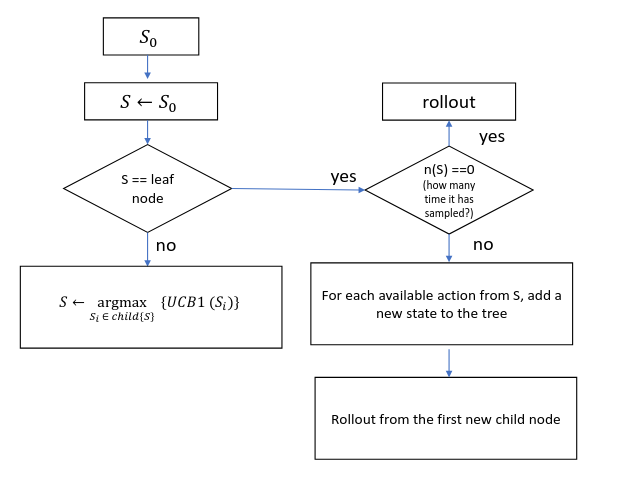
\includegraphics[scale=0.5]{prob5_flow_chart.png}
    \end{figure}

    Now, let us describe how we use the above flow chart to balance exploration and exploitation.
    At first, we just have the root node, $S_0$. This technically currently a leaf node, but
    since it is the root-node, we make an exception and immediately add new child nodes to it,
    and rollout from the first new child node. Based on the results of the rollout, we update
    the value of the first new child node and its parent.\\

    Then, we restart the algorithm from the root node. This time, since the root node is no longer
    a leaf node, we need to use UCB1 to select a leaf node. Now this is where the exploration-exploitation
    trade-off comes in. We will find that even though the first new child node has a high value (since
    we rolled out from it previously), it would be the choice in case of greedy selection. However,
    since we are using UCB1, we will instead consider the second new child node, which has a lower value,
    because its exploration term is higher. Specifically, the exploration term is higher because $n_i$ is
    0, making the second term in the UCB1 for that node infinitely large. This shows that in the planning
    phase, MCTS balances exploration and exploitation by using the UCB1 formula.\\


\end{homeworkProblem}

\end{document}